\documentclass[]{article}
\usepackage{lmodern}
\usepackage{amssymb,amsmath}
\usepackage{ifxetex,ifluatex}
\usepackage{fixltx2e} % provides \textsubscript
\ifnum 0\ifxetex 1\fi\ifluatex 1\fi=0 % if pdftex
  \usepackage[T1]{fontenc}
  \usepackage[utf8]{inputenc}
\else % if luatex or xelatex
  \ifxetex
    \usepackage{mathspec}
  \else
    \usepackage{fontspec}
  \fi
  \defaultfontfeatures{Ligatures=TeX,Scale=MatchLowercase}
    \setmonofont[Mapping=tex-ansi,Scale=0.7]{Source Code Pro}
\fi
% use upquote if available, for straight quotes in verbatim environments
\IfFileExists{upquote.sty}{\usepackage{upquote}}{}
% use microtype if available
\IfFileExists{microtype.sty}{%
\usepackage{microtype}
\UseMicrotypeSet[protrusion]{basicmath} % disable protrusion for tt fonts
}{}
\usepackage[margin=1in]{geometry}
\usepackage{hyperref}
\PassOptionsToPackage{usenames,dvipsnames}{color} % color is loaded by hyperref
\hypersetup{unicode=true,
            pdftitle={ANS performance briefing - UK},
            pdfauthor={EUROCONTROL Performance Review Unit},
            colorlinks=true,
            linkcolor=Maroon,
            citecolor=Blue,
            urlcolor=blue,
            breaklinks=true}
\urlstyle{same}  % don't use monospace font for urls
\usepackage{longtable,booktabs}
\usepackage{graphicx,grffile}
\makeatletter
\def\maxwidth{\ifdim\Gin@nat@width>\linewidth\linewidth\else\Gin@nat@width\fi}
\def\maxheight{\ifdim\Gin@nat@height>\textheight\textheight\else\Gin@nat@height\fi}
\makeatother
% Scale images if necessary, so that they will not overflow the page
% margins by default, and it is still possible to overwrite the defaults
% using explicit options in \includegraphics[width, height, ...]{}
\setkeys{Gin}{width=\maxwidth,height=\maxheight,keepaspectratio}
\IfFileExists{parskip.sty}{%
\usepackage{parskip}
}{% else
\setlength{\parindent}{0pt}
\setlength{\parskip}{6pt plus 2pt minus 1pt}
}
\setlength{\emergencystretch}{3em}  % prevent overfull lines
\providecommand{\tightlist}{%
  \setlength{\itemsep}{0pt}\setlength{\parskip}{0pt}}
\setcounter{secnumdepth}{5}

%%% Use protect on footnotes to avoid problems with footnotes in titles
\let\rmarkdownfootnote\footnote%
\def\footnote{\protect\rmarkdownfootnote}

%%% Change title format to be more compact
\usepackage{titling}

% Create subtitle command for use in maketitle
\providecommand{\subtitle}[1]{
  \posttitle{
    \begin{center}\large#1\end{center}
    }
}

\setlength{\droptitle}{-2em}

  \title{ANS performance briefing - UK}
    \pretitle{\vspace{\droptitle}\centering\huge}
  \posttitle{\par}
    \author{EUROCONTROL Performance Review Unit}
    \preauthor{\centering\large\emph}
  \postauthor{\par}
      \predate{\centering\large\emph}
  \postdate{\par}
    \date{08/Aug/2019}

\usepackage{float}
\floatplacement{figure}{H}

\begin{document}
\maketitle

\begin{center}
\includegraphics[width=\textwidth]{images/logo} \end{center}

\newpage

\hypertarget{preface}{%
\section*{Preface}\label{preface}}
\addcontentsline{toc}{section}{Preface}

This performance briefing has been prepared by the EUROCONTROL Performance Review Unit (PRU) in the interest of the exchange of information.

If you have any questions related to this document or if we can help with any ANS performance related matter, then please do not hesitate to contact us: \href{mailto:pru-support@eurocontrol.int}{\nolinkurl{pru-support@eurocontrol.int}}

The information may be copied in whole or in part providing that the copyright notice and disclaimer are included.

The views expressed herein do not necessarily reflect the official views or policy of EUROCONTROL, which makes no warranty, either implied or express, for the information contained in this document, neither does it assume any legal liability or responsibility for the accuracy, completeness or usefulness of this information.

\newpage

\hypertarget{key-observations}{%
\section*{Key observations}\label{key-observations}}
\addcontentsline{toc}{section}{Key observations}

\hypertarget{traffic}{%
\subsection*{TRAFFIC}\label{traffic}}
\addcontentsline{toc}{subsection}{TRAFFIC}

\begin{itemize}
\item
  Following the high traffic increase already in 2017 ..
\item
  The strong growth ..
\item
  As a result ..
\end{itemize}

\hypertarget{safety}{%
\subsection*{SAFETY}\label{safety}}
\addcontentsline{toc}{subsection}{SAFETY}

\begin{itemize}
\tightlist
\item
  No data available
\end{itemize}

\hypertarget{capacity}{%
\subsection*{CAPACITY}\label{capacity}}
\addcontentsline{toc}{subsection}{CAPACITY}

\hypertarget{en-route-atfm-delays}{%
\subsubsection*{En-route ATFM delays}\label{en-route-atfm-delays}}
\addcontentsline{toc}{subsubsection}{En-route ATFM delays}

\begin{itemize}
\tightlist
\item
  No en-route ATFM delay..
\end{itemize}

\hypertarget{airport-arrival-atfm-delays}{%
\subsubsection*{Airport arrival ATFM delays}\label{airport-arrival-atfm-delays}}
\addcontentsline{toc}{subsubsection}{Airport arrival ATFM delays}

\begin{itemize}
\tightlist
\item
  No airport arrival ATFM delay..
\end{itemize}

\hypertarget{environment}{%
\subsection*{ENVIRONMENT}\label{environment}}
\addcontentsline{toc}{subsection}{ENVIRONMENT}

\hypertarget{horizontal-en-route-flight-efficiency}{%
\subsubsection*{Horizontal en-route flight efficiency}\label{horizontal-en-route-flight-efficiency}}
\addcontentsline{toc}{subsubsection}{Horizontal en-route flight efficiency}

\begin{itemize}
\tightlist
\item
  In 2008, Finland..
\end{itemize}

\hypertarget{vertical-en-route-flight-efficiency}{%
\subsubsection*{Vertical en-route flight efficiency}\label{vertical-en-route-flight-efficiency}}
\addcontentsline{toc}{subsubsection}{Vertical en-route flight efficiency}

\hypertarget{vertical-flight-efficiency-during-climb-and-descent}{%
\subsubsection*{Vertical flight efficiency during climb and descent}\label{vertical-flight-efficiency-during-climb-and-descent}}
\addcontentsline{toc}{subsubsection}{Vertical flight efficiency during climb and descent}

\hypertarget{cost-effectiveness}{%
\subsection*{COST-EFFECTIVENESS}\label{cost-effectiveness}}
\addcontentsline{toc}{subsection}{COST-EFFECTIVENESS}

\begin{itemize}
\item
  ARMATS represents.. see {[}\protect\hyperlink{ref-pru:ace-report-2015}{1}{]}
\item
  Since ARMATS did not..
\item
  Compared to the..
\end{itemize}

\newpage

% Trigger ToC creation in LaTeX
\tableofcontents

\newpage

\listoffigures

\newpage

\hypertarget{institutional-arrangements}{%
\section{Institutional arrangements}\label{institutional-arrangements}}

\newpage

\hypertarget{traffic-characteristics}{%
\section{Traffic characteristics}\label{traffic-characteristics}}

Sources: NM; {[}\protect\hyperlink{ref-7year-forecast-2019}{2}{]}

\newpage

\hypertarget{safety-1}{%
\section{Safety}\label{safety-1}}

\newpage

\hypertarget{capacity-1}{%
\section{Capacity}\label{capacity-1}}

\hypertarget{air-traffic-flow-management-atfm-delays}{%
\subsection{Air traffic flow management (ATFM) delays}\label{air-traffic-flow-management-atfm-delays}}

Source : NM, PRU ANS Performance Data Portal\\
The data in this section is from the PRU ANS performance data portal (data section).\\
It is available at: \url{http://ansperformance.eu/data/performancearea/}

\hypertarget{en-route-atfm-delays-1}{%
\subsubsection{En-route ATFM delays}\label{en-route-atfm-delays-1}}

\begin{figure}

{\centering 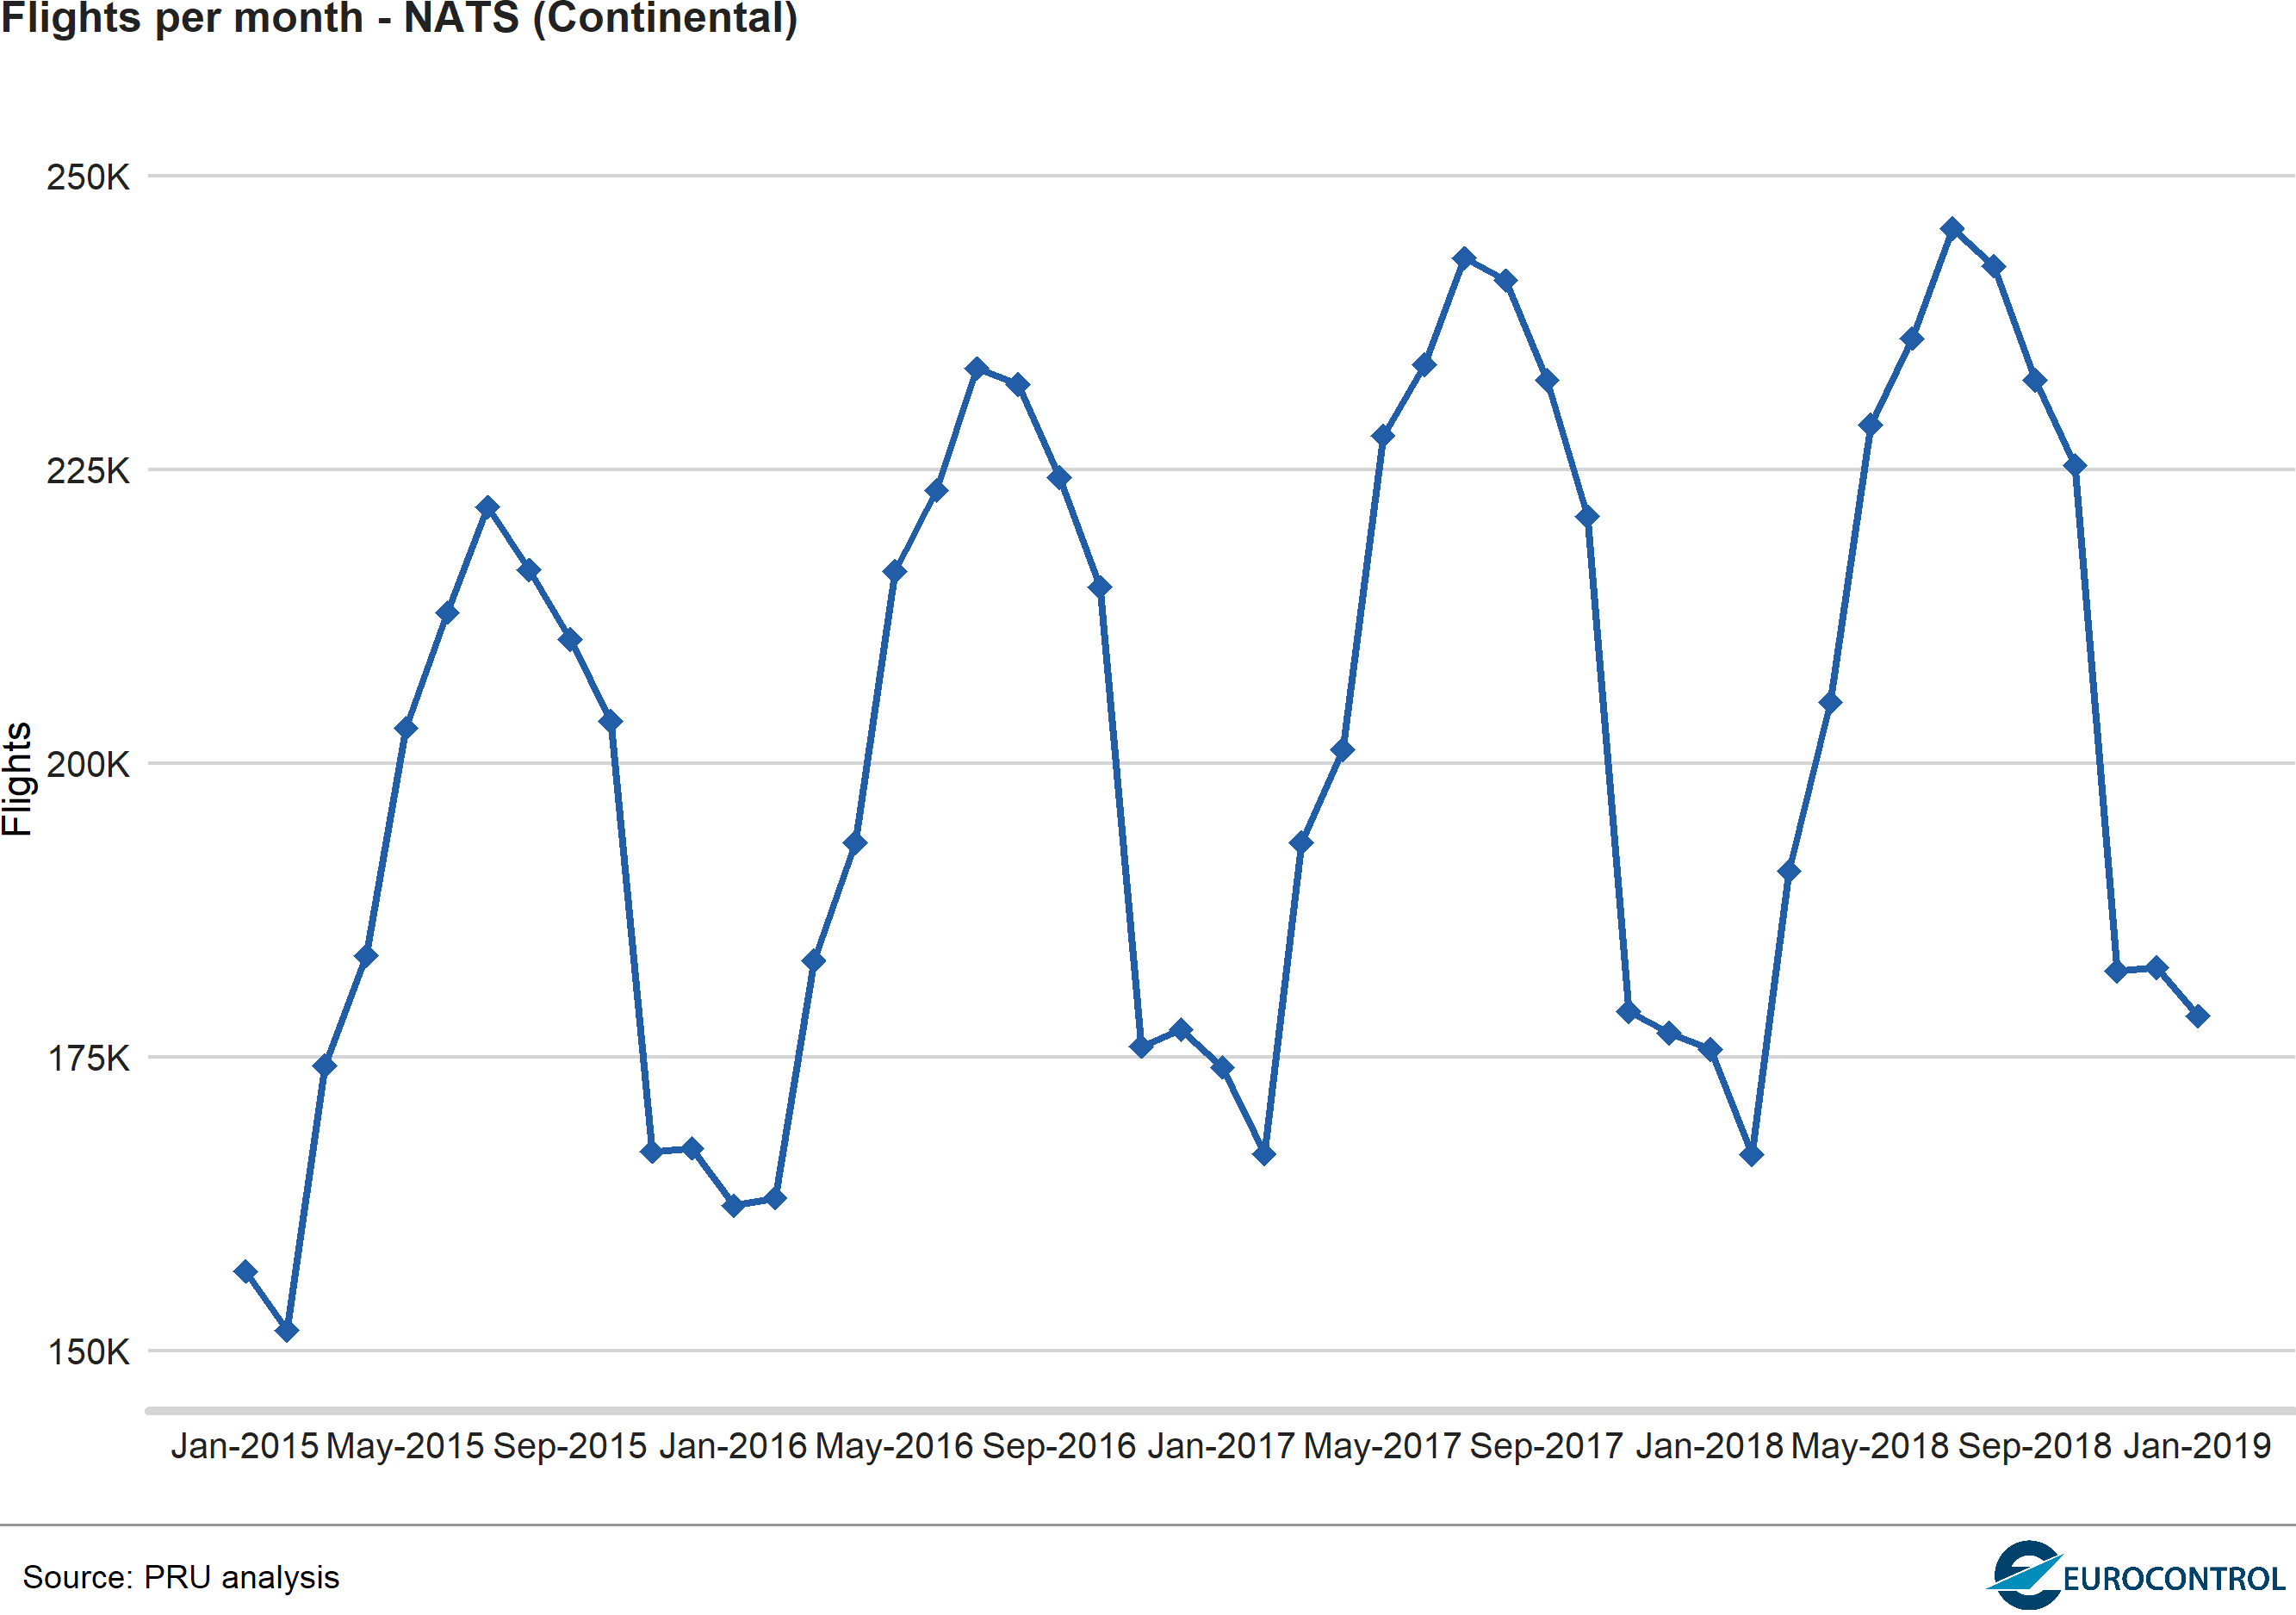
\includegraphics[width=\textwidth]{G:/HQ/dgof-pru/Project/Vertical_flight_efficiency/2015/State_briefing/Figures/Nbr_flights_NATS (Continental)} 

}

\caption{Number of flights}(\#fig:enr-flights)
\end{figure}

\begin{figure}

{\centering 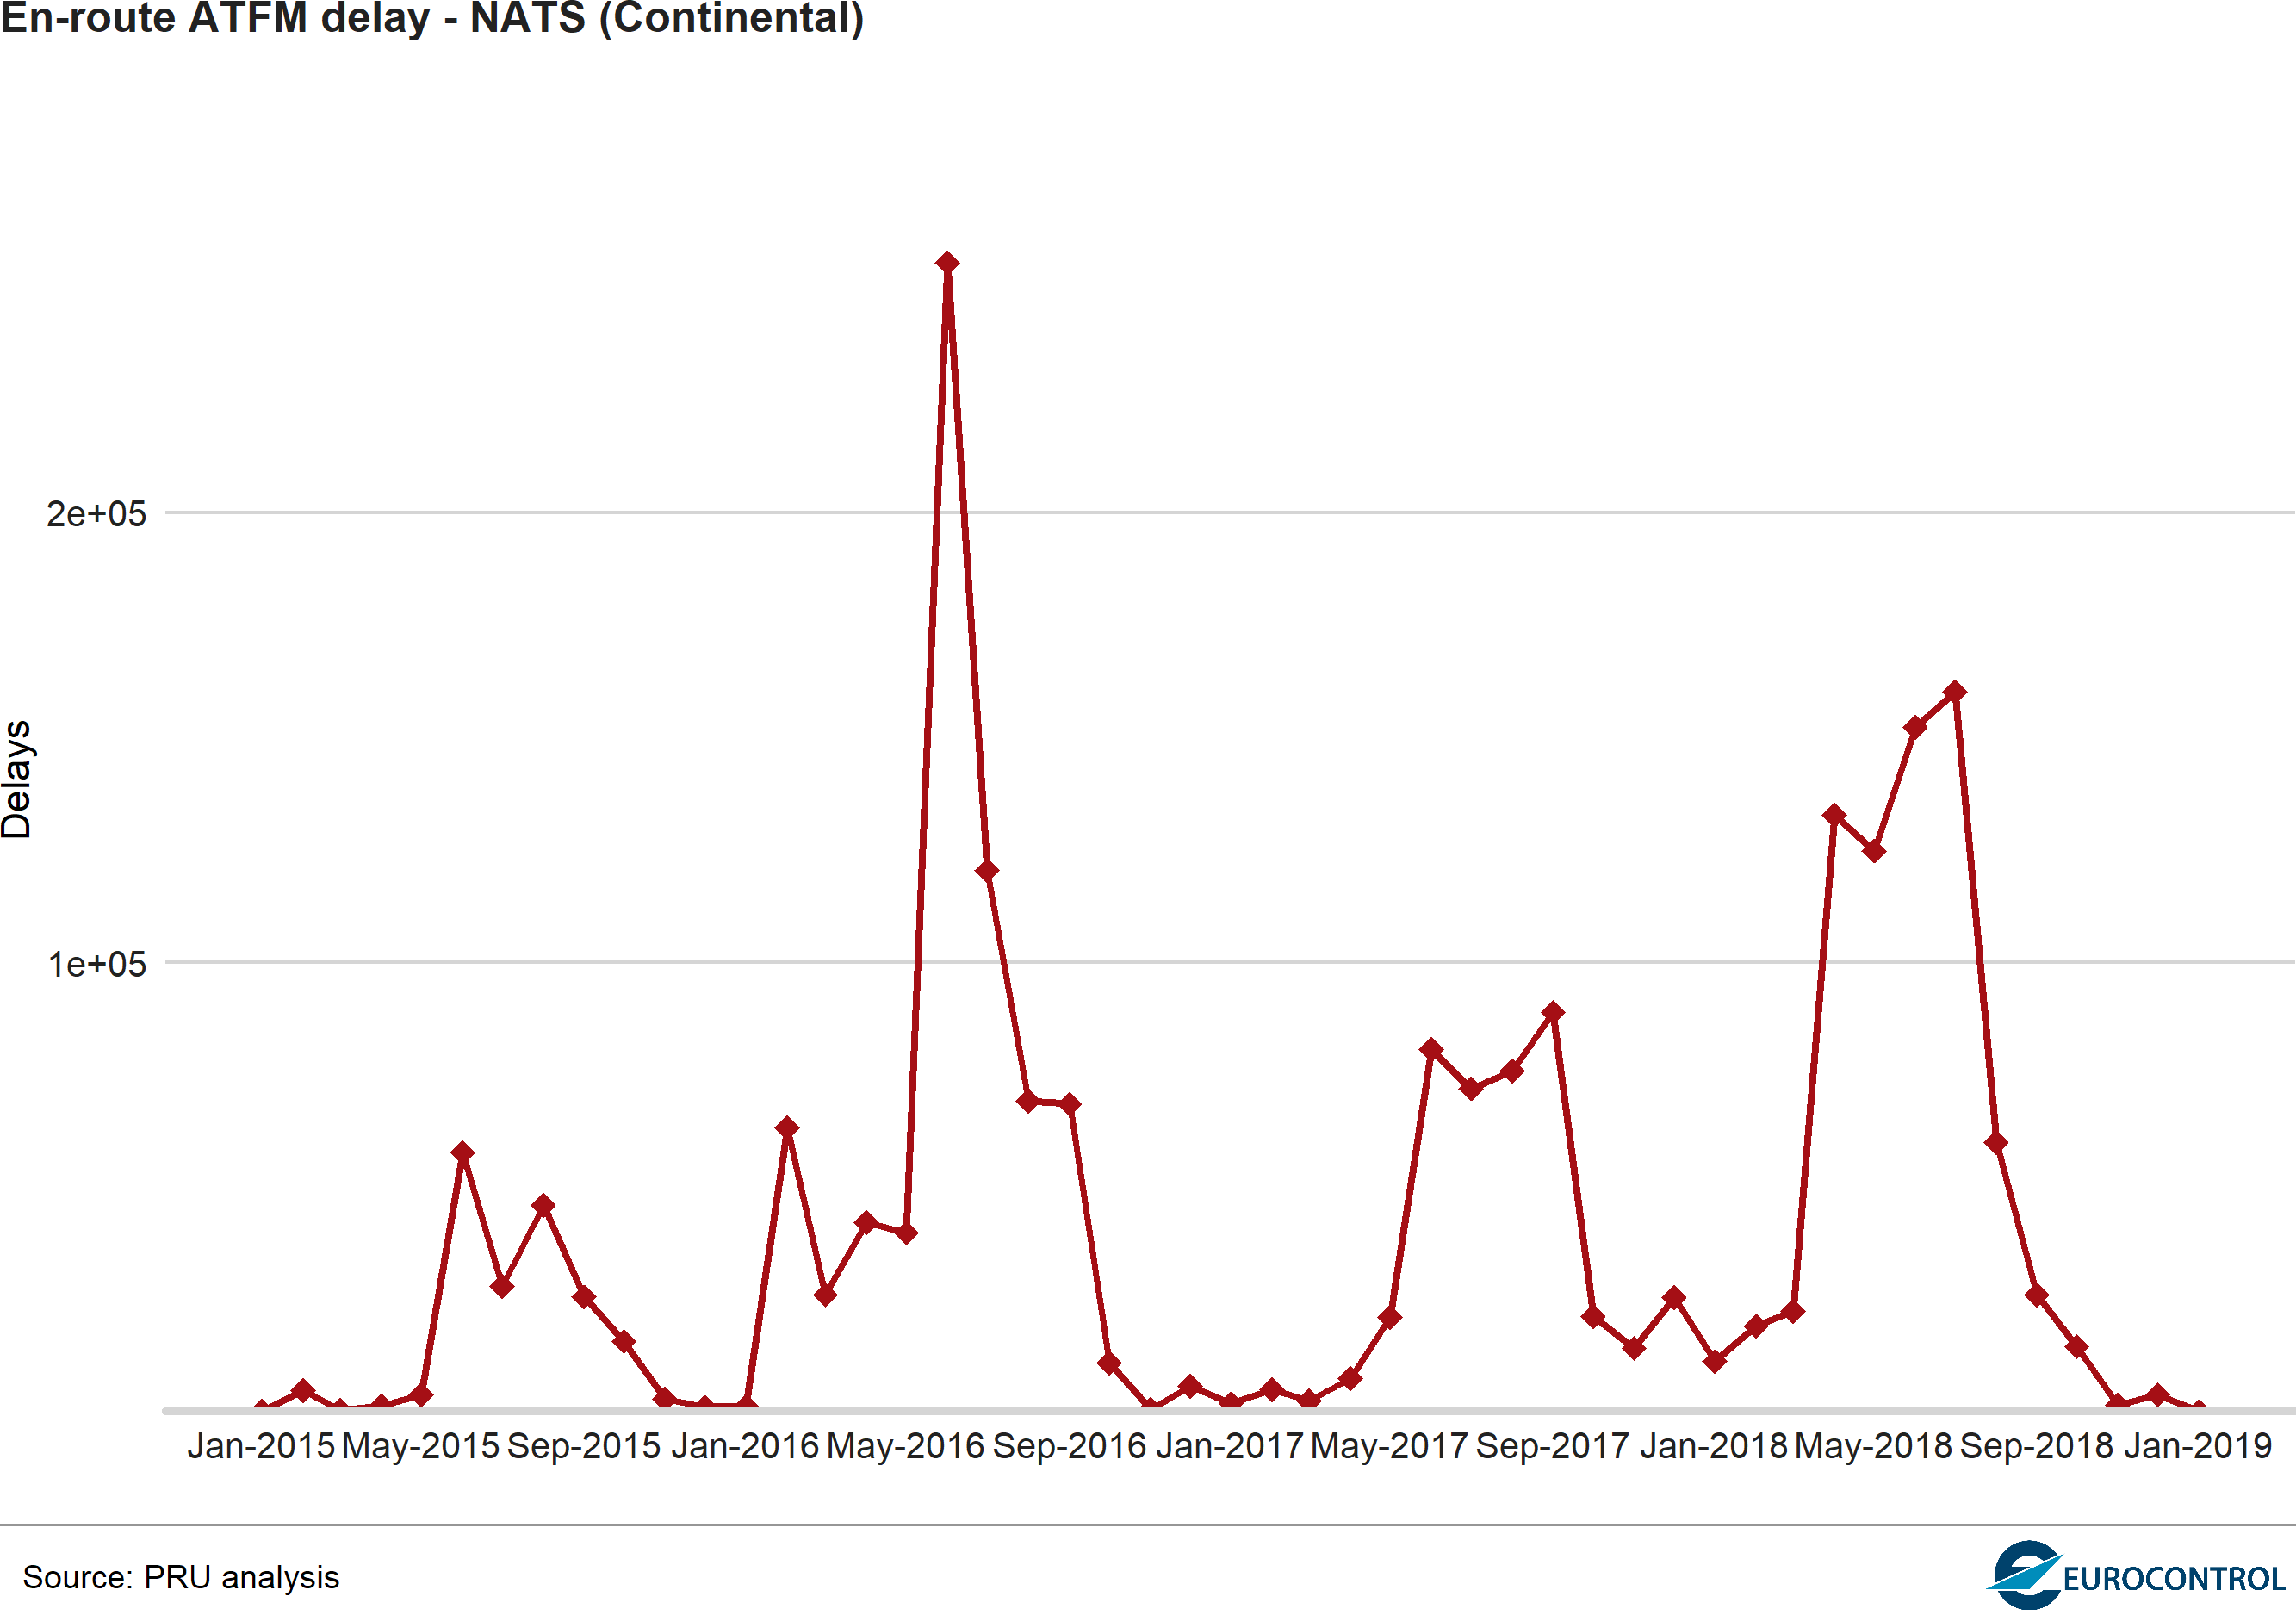
\includegraphics[width=\textwidth]{G:/HQ/dgof-pru/Project/Vertical_flight_efficiency/2015/State_briefing/Figures/ENR_ATFM_delays_NATS (Continental)} 

}

\caption{En-route ATFM delay}(\#fig:enr-delay)
\end{figure}

\begin{figure}

{\centering 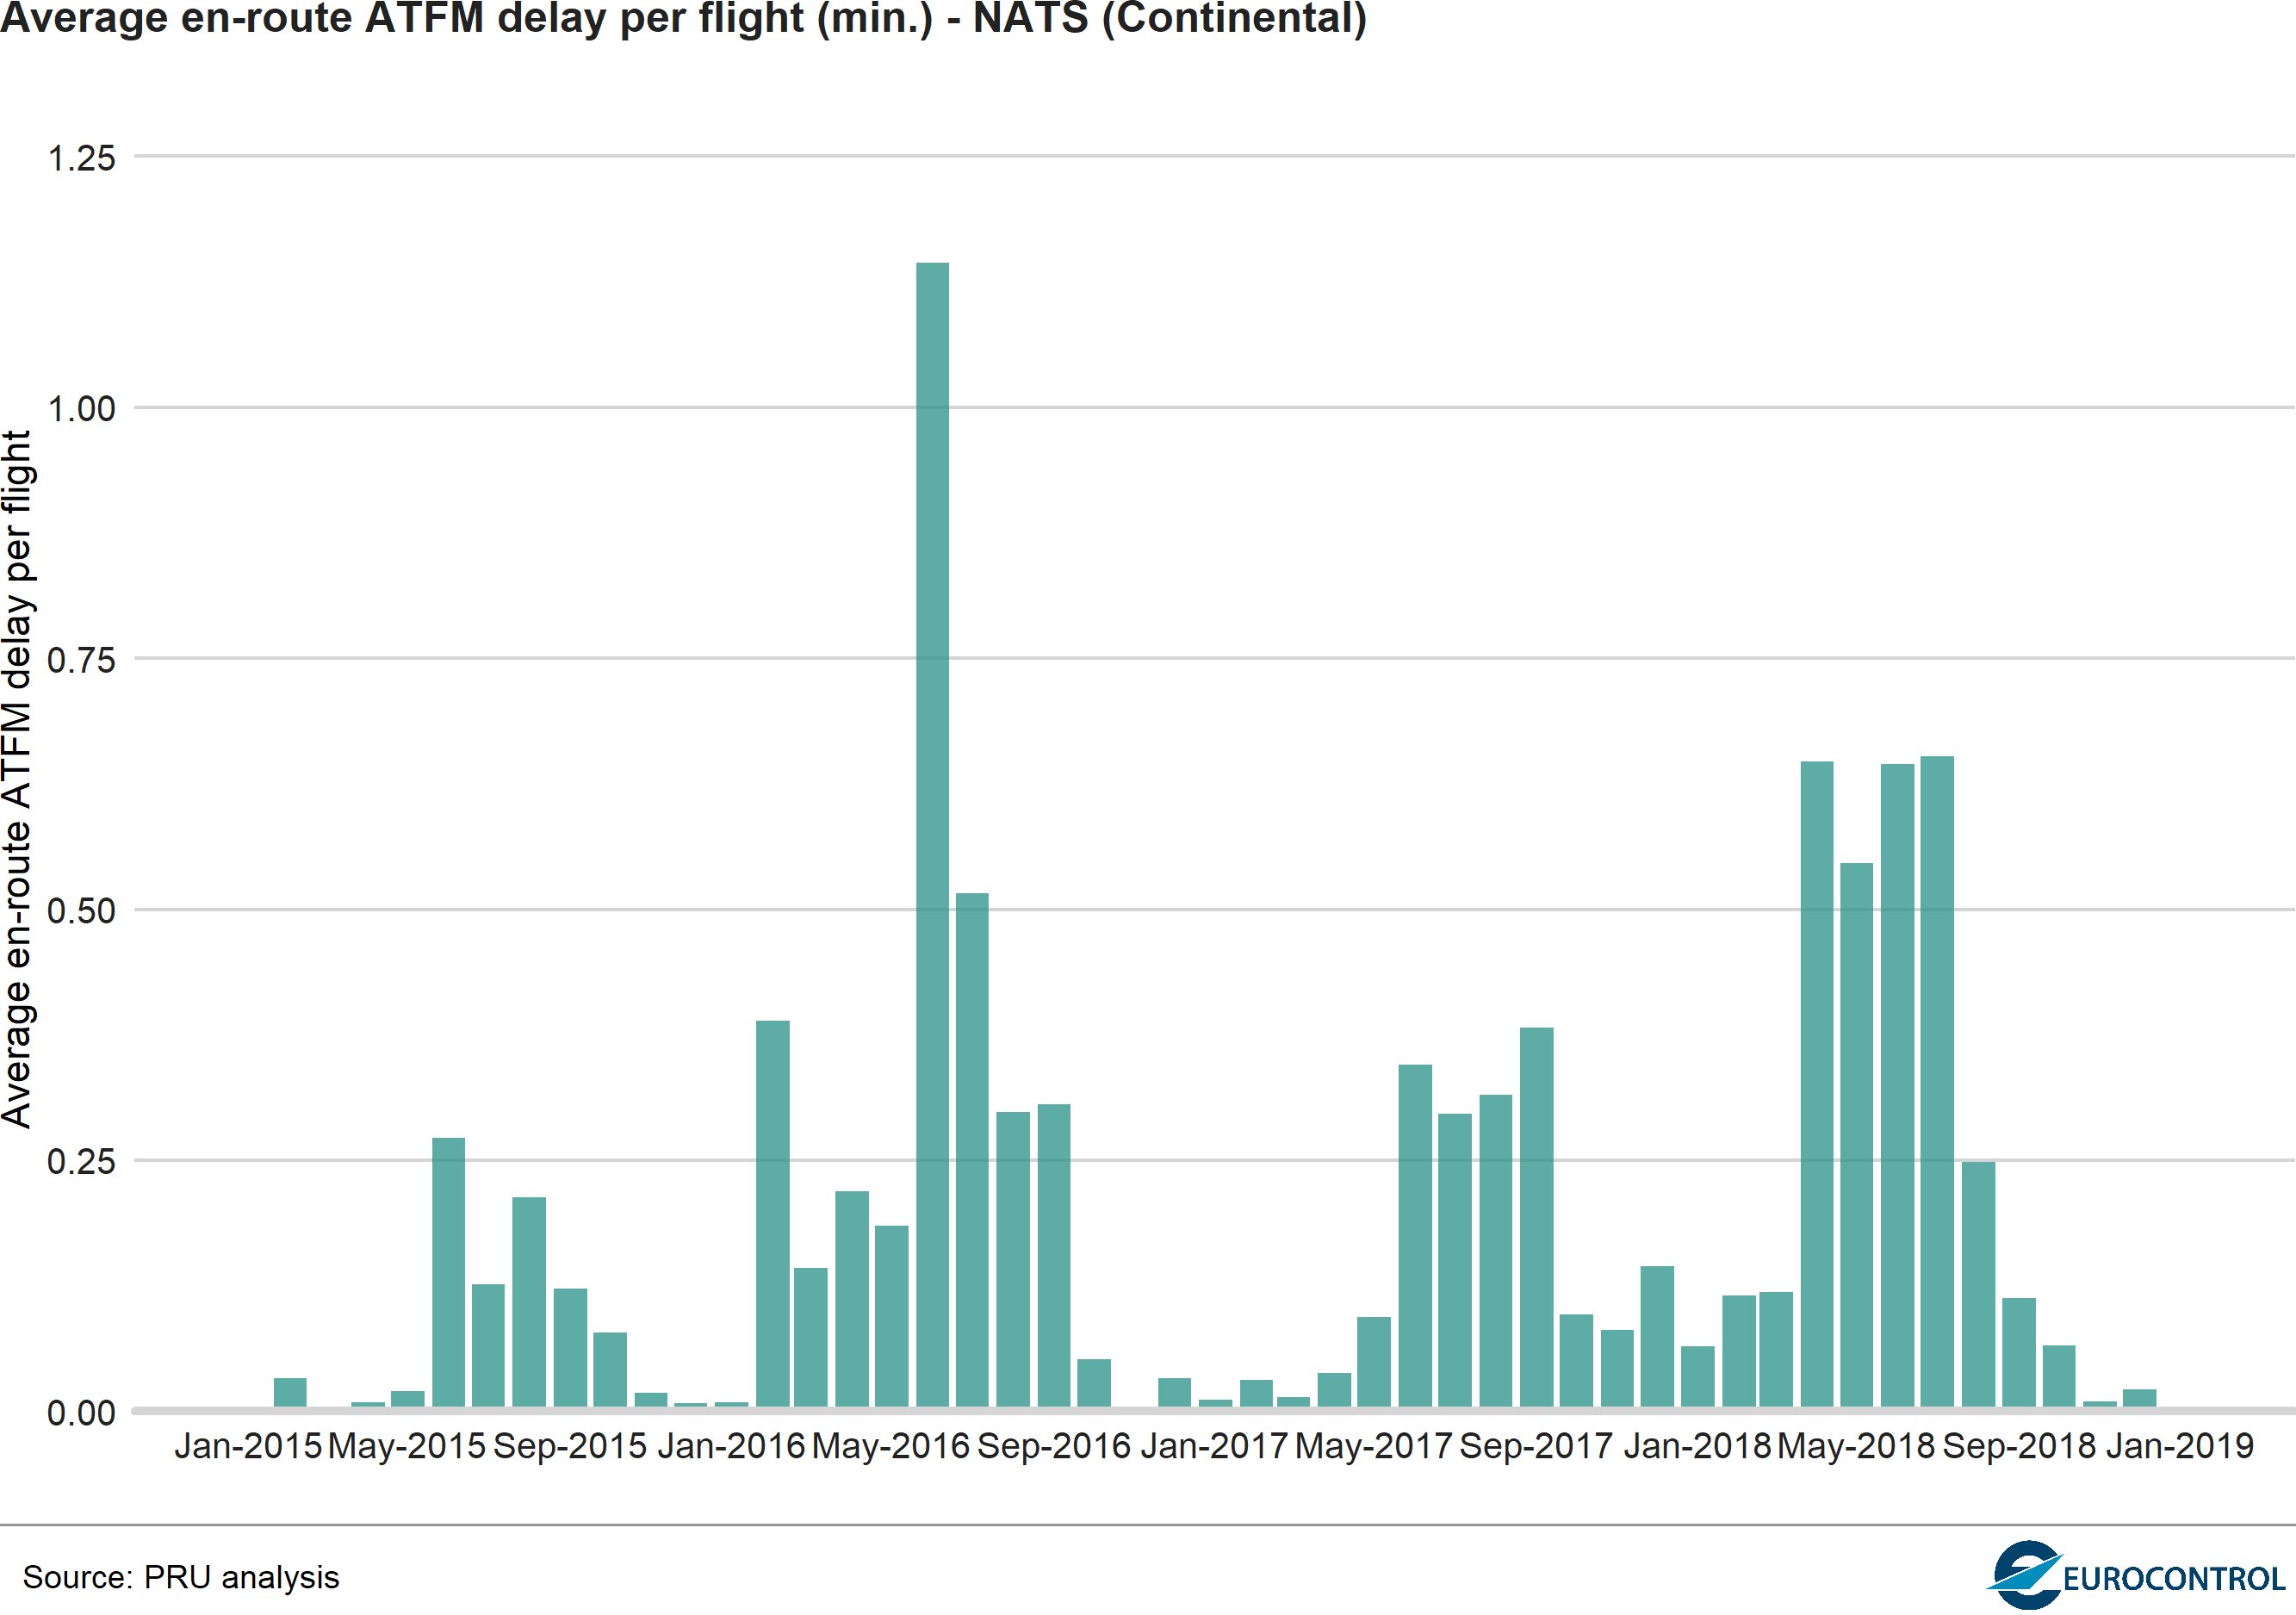
\includegraphics[width=\textwidth]{G:/HQ/dgof-pru/Project/Vertical_flight_efficiency/2015/State_briefing/Figures/Avg_ENR_ATFM_delay_flight_NATS (Continental)} 

}

\caption{Average en-route ATFM delay per flight}(\#fig:enr-avg-dly-flt)
\end{figure}

\begin{figure}

{\centering 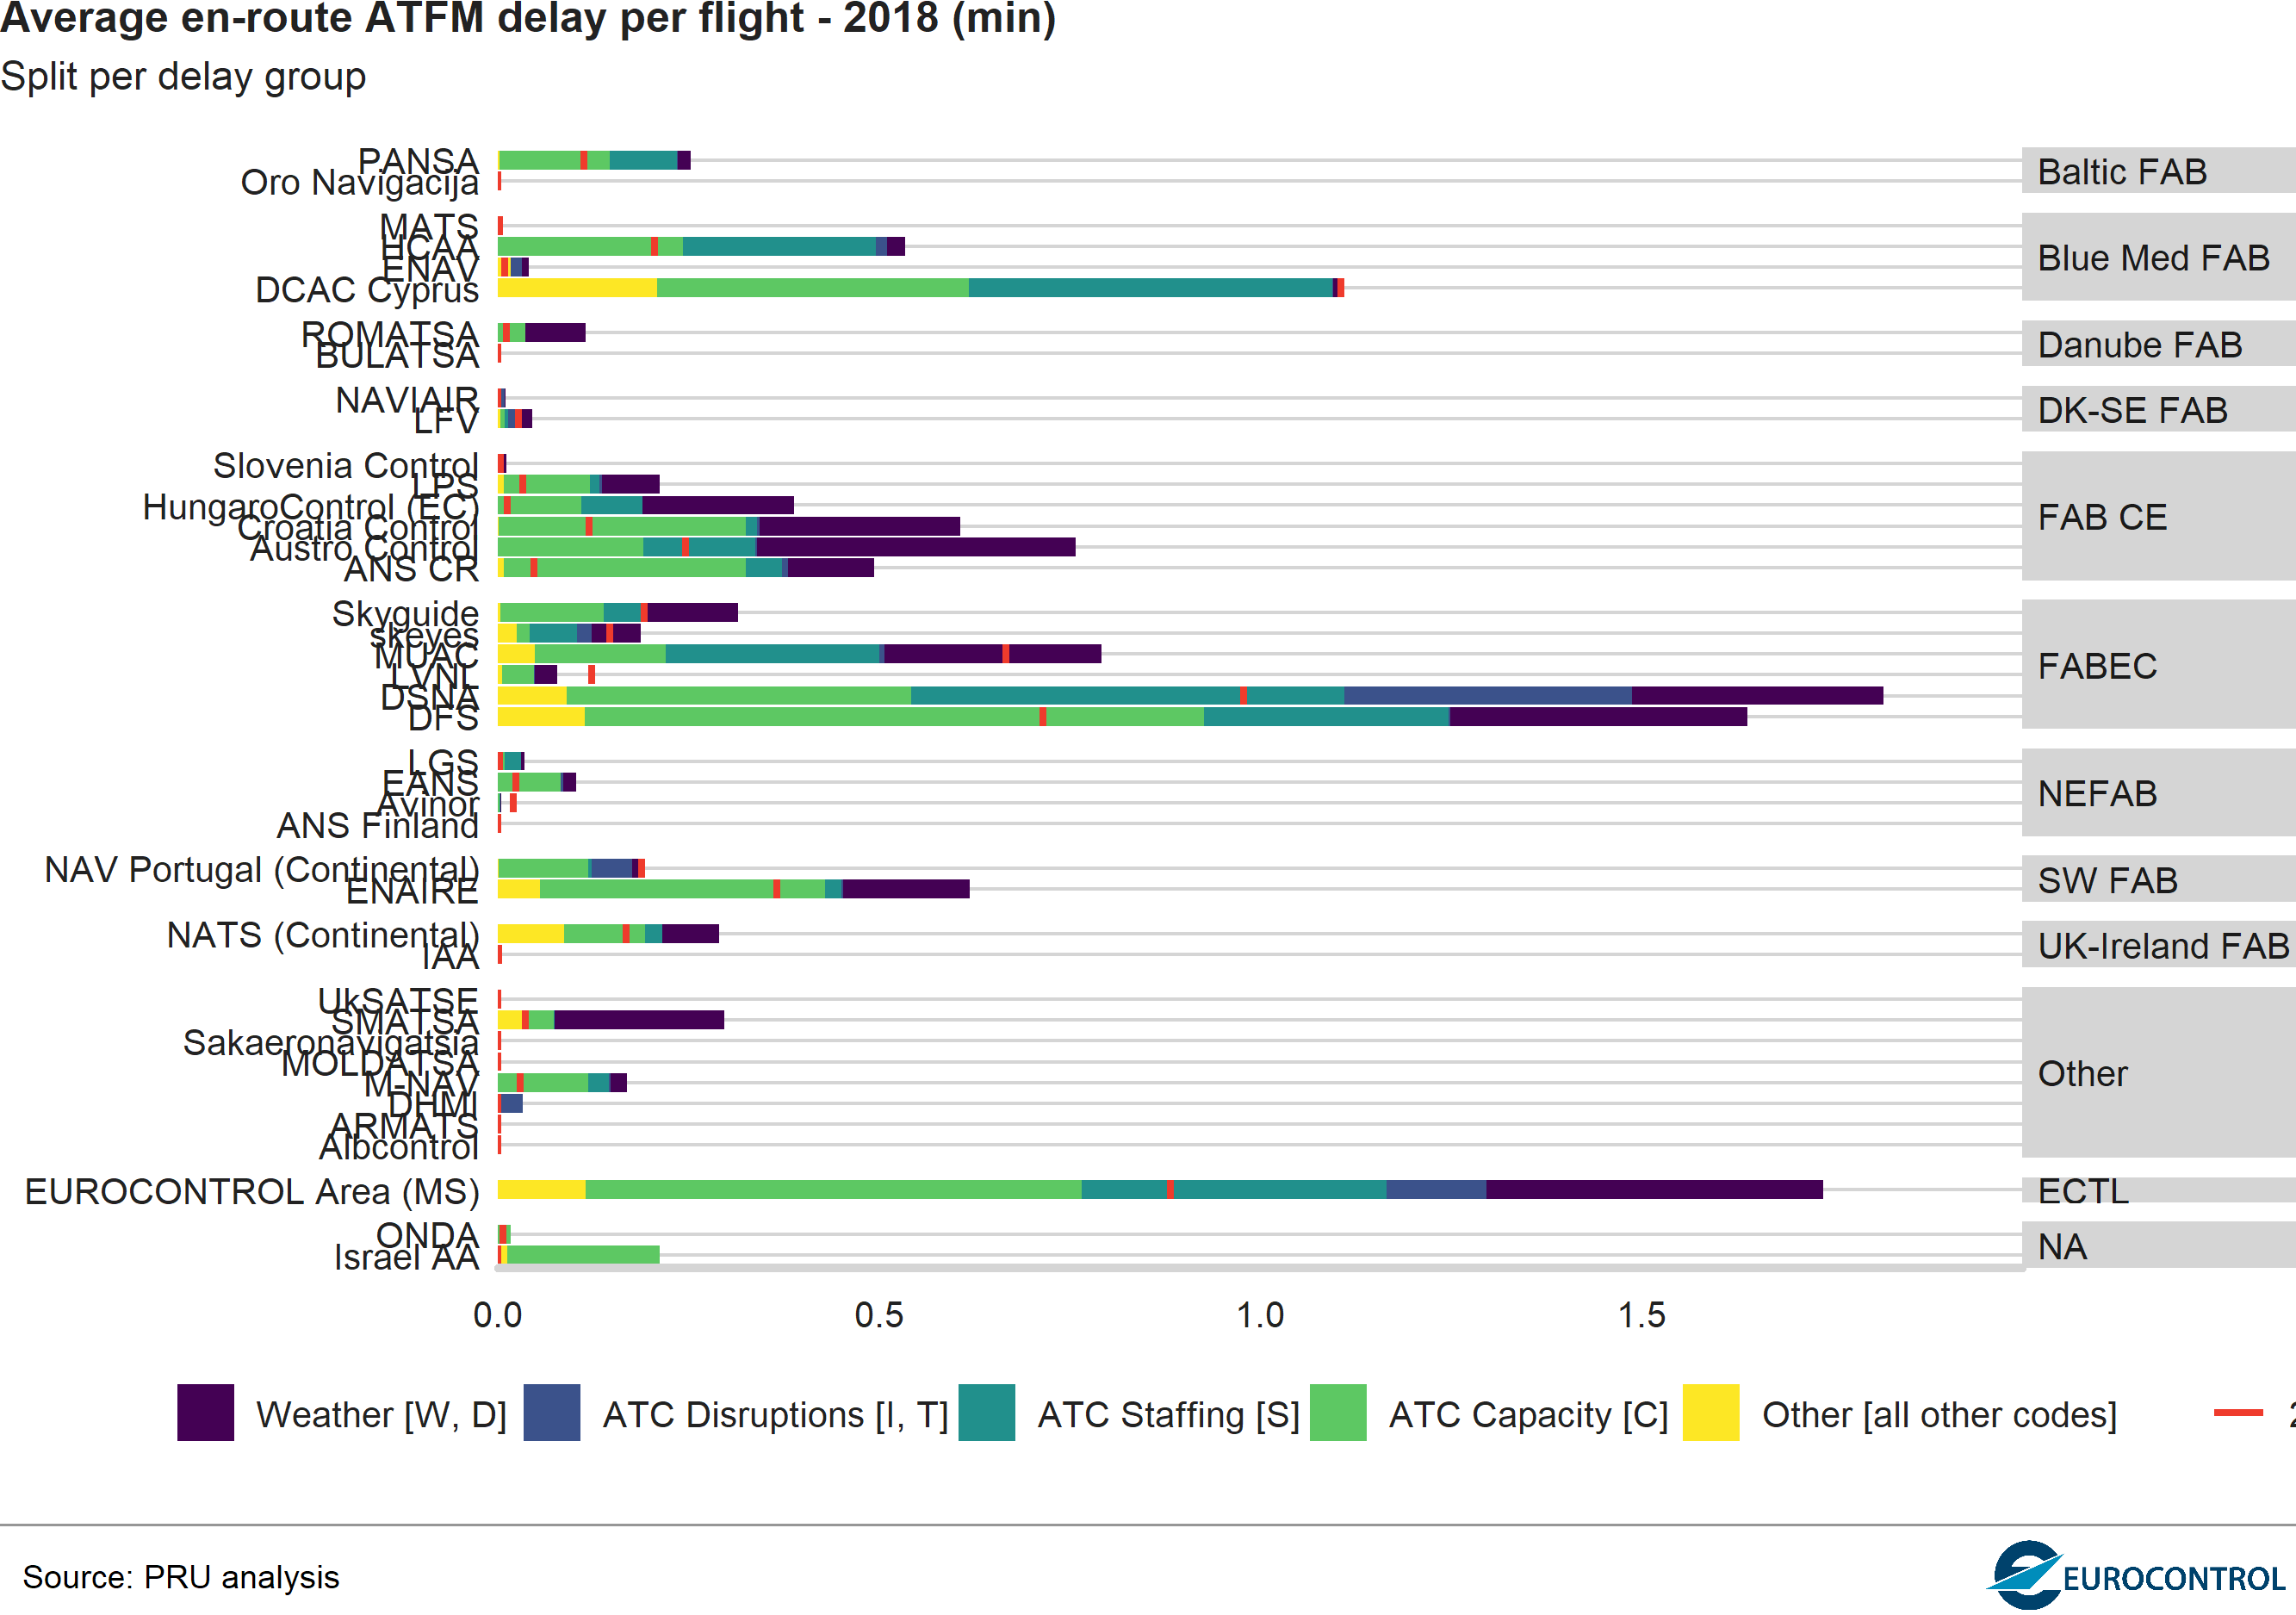
\includegraphics[width=\textwidth]{G:/HQ/dgof-pru/Project/Vertical_flight_efficiency/2015/State_briefing/Figures/Avg_ENR_ATFM_delay_flight_group_NATS (Continental)} 

}

\caption{Average en route ATFM delay per flight (EUROCONTROL area)}(\#fig:enr-average-delay-grouped)
\end{figure}

\hypertarget{airport-arrival-atfm-delays-1}{%
\subsubsection{Airport arrival ATFM delays}\label{airport-arrival-atfm-delays-1}}

\hypertarget{environment-1}{%
\section{Environment}\label{environment-1}}

Source : PRU ANS Performance Data Portal
The data in this section is from the PRU ANS performance data portal (data section).\\
It is available at: \url{http://ansperformance.eu/data/performancearea/}

\hypertarget{horizontal-flight-efficiency}{%
\subsection{Horizontal flight efficiency}\label{horizontal-flight-efficiency}}

(ref:hfe-year) Horizontal en-route flight efficiency - (NATS (Continental)).

\begin{figure}

{\centering \includegraphics[width=\textwidth]{G:/HQ/dgof-pru/Project/Vertical_flight_efficiency/2015/State_briefing/Figures/HFE_year_NATS (Continental)} 

}

\caption{(ref:hfe-year)}(\#fig:hfe-year)
\end{figure}

(ref:hfe-daily) Horizontal en-route flight efficiency - (NATS (Continental)).

\begin{figure}

{\centering 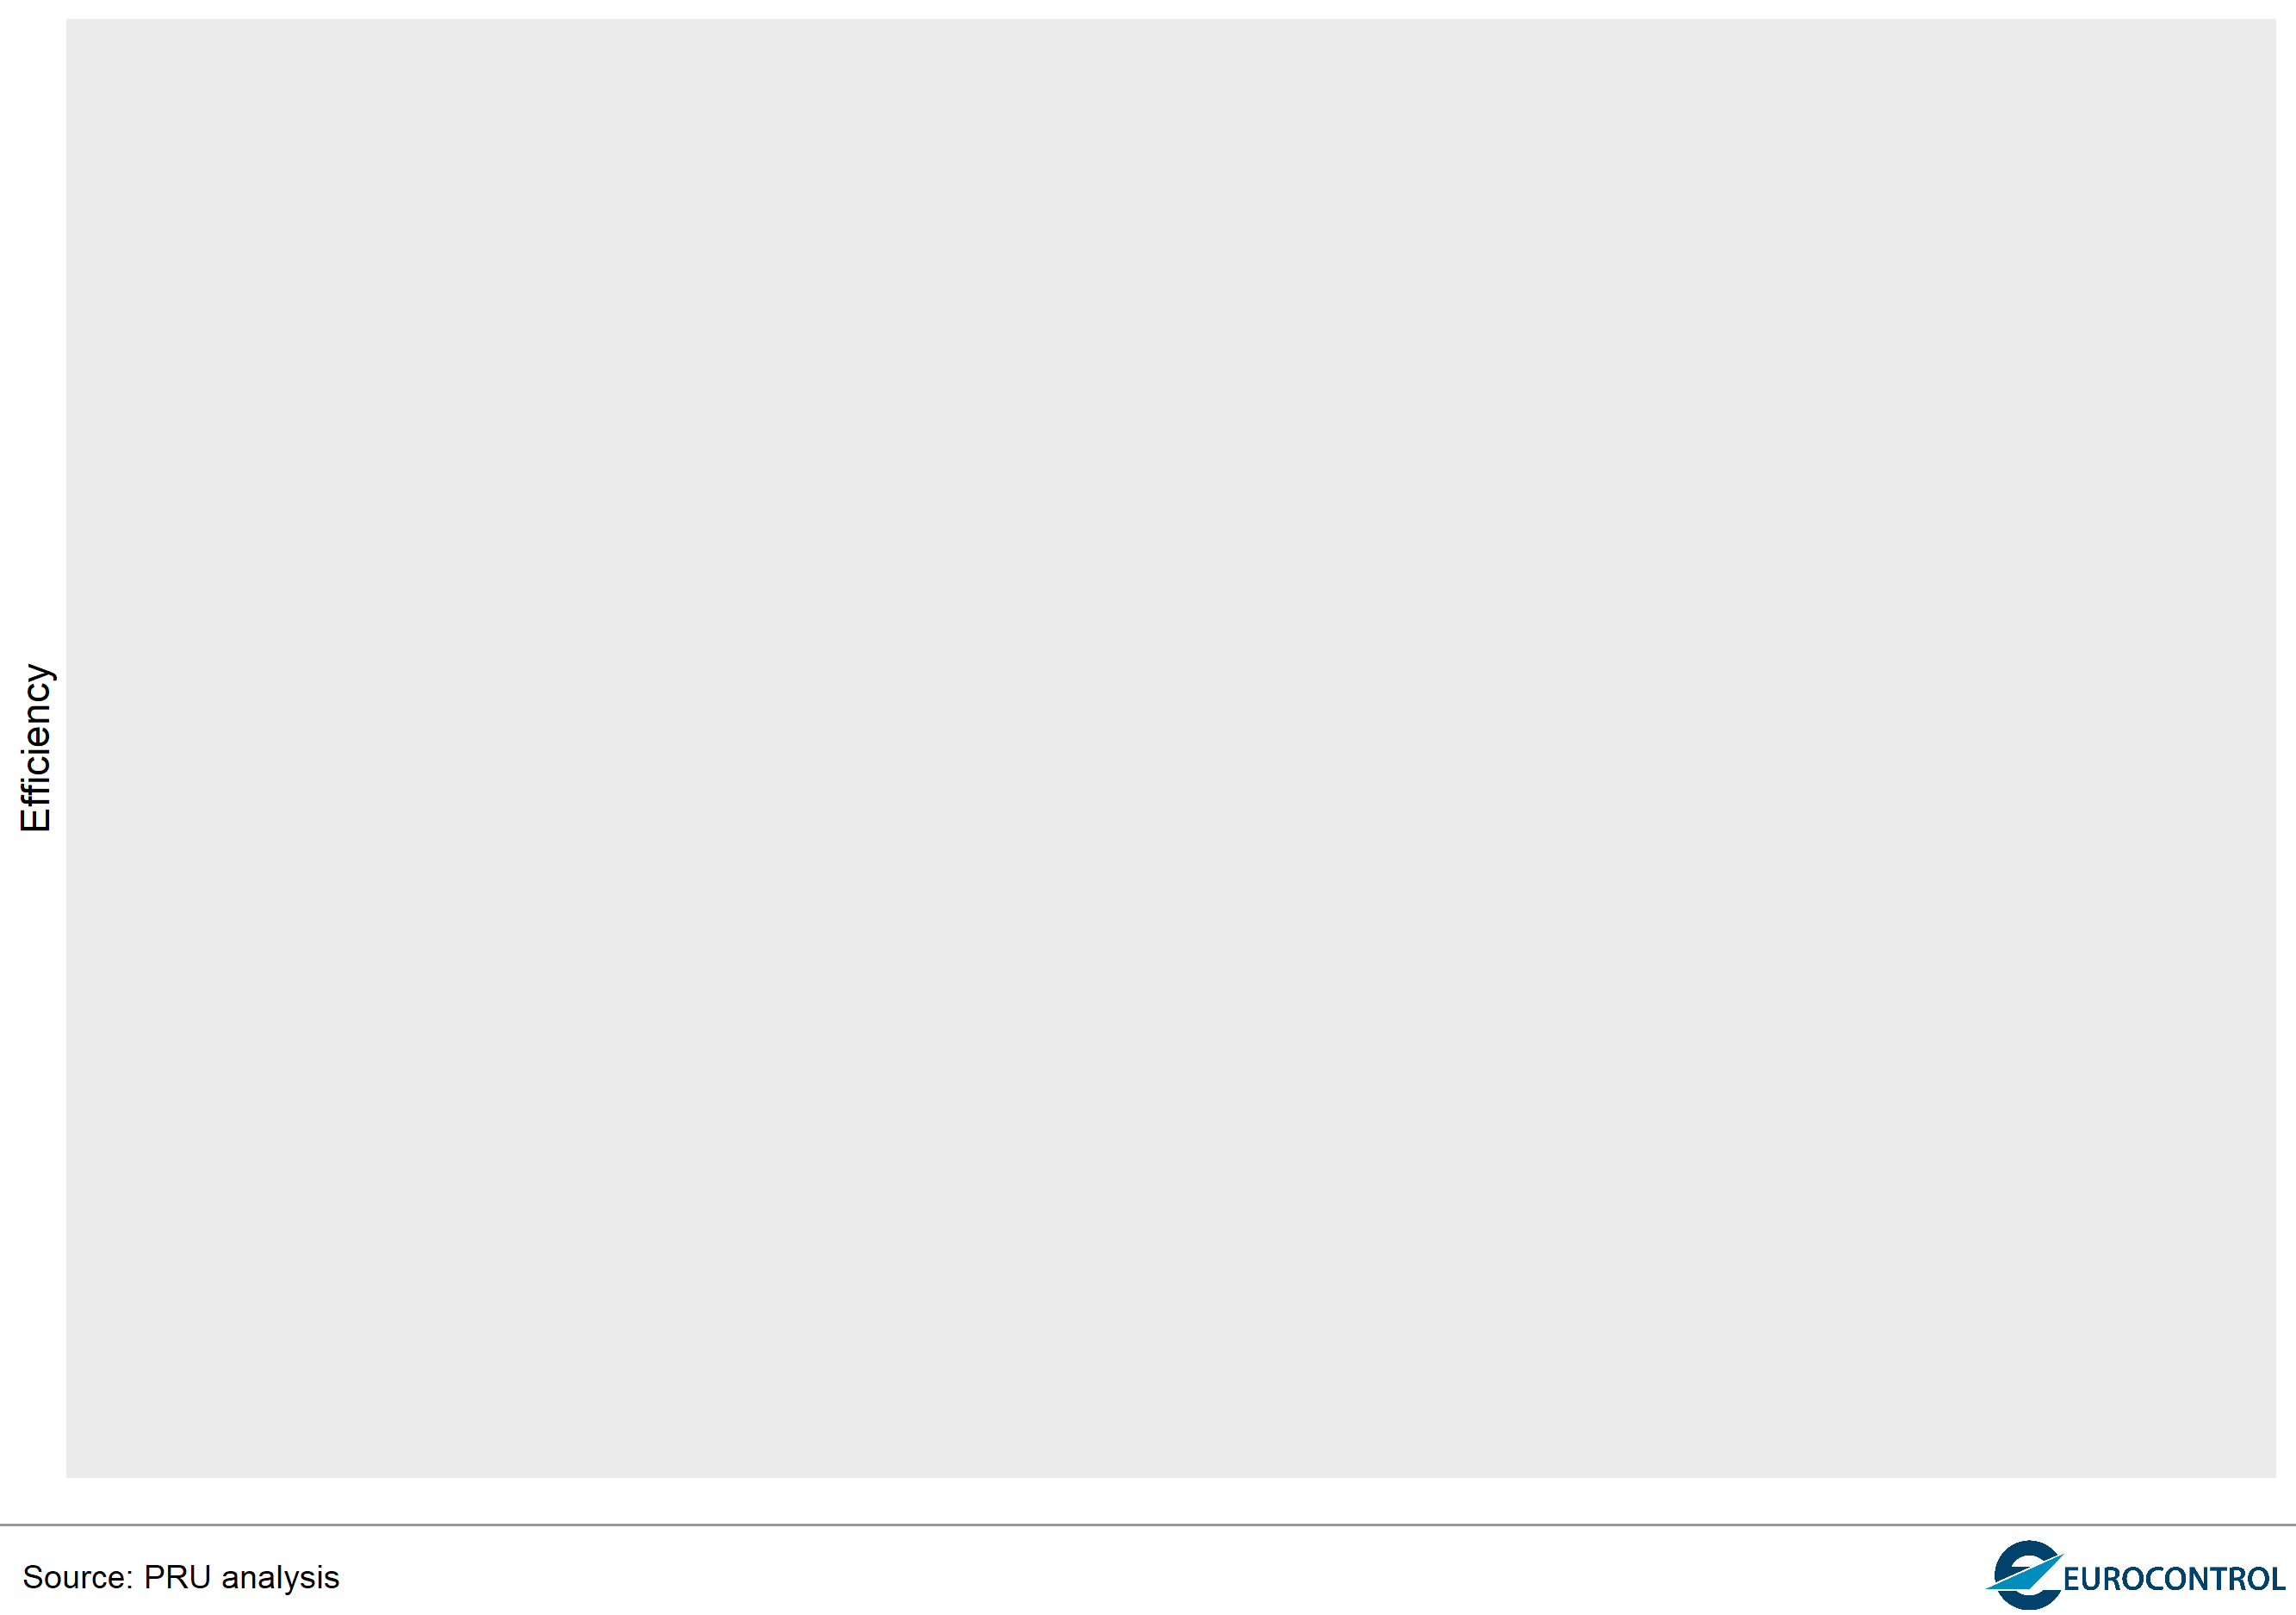
\includegraphics[width=\textwidth]{G:/HQ/dgof-pru/Project/Vertical_flight_efficiency/2015/State_briefing/Figures/HFE_day_NATS (Continental)} 

}

\caption{(ref:hfe-daily)}(\#fig:hfe-daily)
\end{figure}

\begin{itemize}
\tightlist
\item
  Horizontal en-route flight efficiency (actual trajectory) was 91.9\%
  in the EUROCONTROL area in 2018.
\end{itemize}

\newpage

\hypertarget{cost-effectiveness-1}{%
\section{Cost-effectiveness}\label{cost-effectiveness-1}}

\newpage

\hypertarget{annex-1-evolution-of-cost-effectiveness-performance-2012-2017}{%
\section{Annex 1: Evolution of cost-effectiveness performance (2012-2017)}\label{annex-1-evolution-of-cost-effectiveness-performance-2012-2017}}

\newpage

\hypertarget{annex-2-network-operations-plan-2018-201922}{%
\section{Annex 2: Network Operations Plan (2018-2019/22)}\label{annex-2-network-operations-plan-2018-201922}}

\hypertarget{yerevan-acc}{%
\subsection{YEREVAN ACC}\label{yerevan-acc}}

\newpage

\hypertarget{references}{%
\section*{References}\label{references}}
\addcontentsline{toc}{section}{References}

\hypertarget{refs}{}
\leavevmode\hypertarget{ref-pru:ace-report-2015}{}%
{[}1{]} Performance Review Unit, ``ATM cost-effectiveness (ace) 2015 benchmarking report with 2016-2020 outlook,'' EUROCONTROL/PRU, Report, May 2017.

\leavevmode\hypertarget{ref-7year-forecast-2019}{}%
{[}2{]} STATFOR, ``EUROCONTROL seven-year forecast february 2019,'' EUROCONTROL/STATFOR, Report, 2017.


\end{document}
